\documentclass[tikz,border=8pt]{standalone}
\usepackage{amsmath}
\usepackage{braket}

\begin{document}
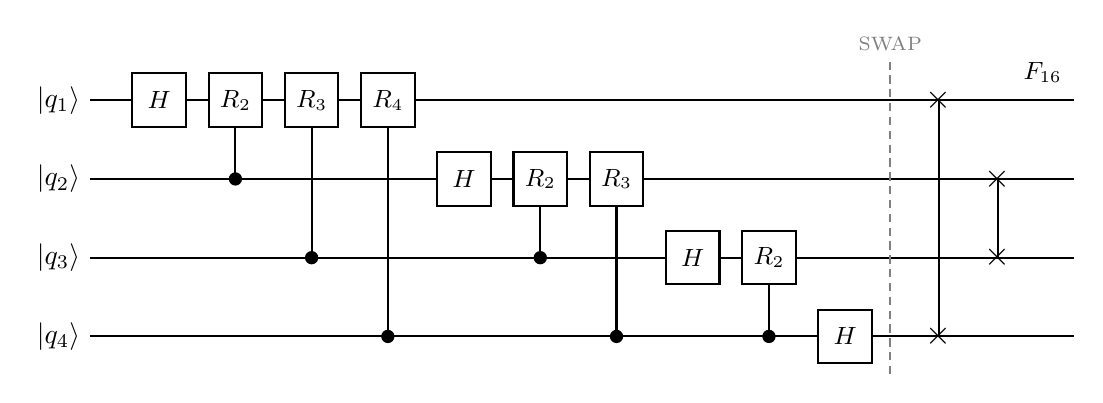
\begin{tikzpicture}[
  x=0.88cm,
  y=1.00cm,
  wire/.style={line width=0.75pt},
  gate/.style={
    draw,
    line width=0.75pt,
    fill=white,
    minimum width=0.68cm,
    minimum height=0.68cm,
    inner sep=0pt,
    font=\small
  },
  control/.style={circle,fill=black,inner sep=1.7pt},
  divider/.style={densely dashed,gray,line width=0.65pt}
]
  % Qubit wires and labels
  \foreach \y/\q in {3/q_1,2/q_2,1/q_3,0/q_4} {
    \draw[wire] (0,\y) -- (14.2,\y);
    \node[left] at (0,\y) {$\ket{\q}$};
  }

  % First output qubit: H followed by controlled R_2, R_3, R_4
  \node[gate] at (1.0,3) {$H$};
  \draw[wire] (2.1,2) -- (2.1,3);
  \node[control] at (2.1,2) {};
  \node[gate] at (2.1,3) {$R_2$};
  \draw[wire] (3.2,1) -- (3.2,3);
  \node[control] at (3.2,1) {};
  \node[gate] at (3.2,3) {$R_3$};
  \draw[wire] (4.3,0) -- (4.3,3);
  \node[control] at (4.3,0) {};
  \node[gate] at (4.3,3) {$R_4$};

  % Second output qubit
  \node[gate] at (5.4,2) {$H$};
  \draw[wire] (6.5,1) -- (6.5,2);
  \node[control] at (6.5,1) {};
  \node[gate] at (6.5,2) {$R_2$};
  \draw[wire] (7.6,0) -- (7.6,2);
  \node[control] at (7.6,0) {};
  \node[gate] at (7.6,2) {$R_3$};

  % Third and fourth output qubits
  \node[gate] at (8.7,1) {$H$};
  \draw[wire] (9.8,0) -- (9.8,1);
  \node[control] at (9.8,0) {};
  \node[gate] at (9.8,1) {$R_2$};
  \node[gate] at (10.9,0) {$H$};

  % Bit-reversal stage
  \draw[divider] (11.55,-0.48) -- (11.55,3.48);
  \node[font=\scriptsize,gray] at (11.55,3.72) {SWAP};

  \draw[wire] (12.25,0) -- (12.25,3);
  \node[font=\large,inner sep=0pt] at (12.25,3) {$\times$};
  \node[font=\large,inner sep=0pt] at (12.25,0) {$\times$};

  \draw[wire] (13.10,1) -- (13.10,2);
  \node[font=\large,inner sep=0pt] at (13.10,2) {$\times$};
  \node[font=\large,inner sep=0pt] at (13.10,1) {$\times$};

  \node[above,font=\small] at (13.75,3.1) {$F_{16}$};
\end{tikzpicture}
\end{document}
